\documentclass[runningheads,a4paper]{llncs}

\usepackage{amssymb}
\usepackage{graphicx}
\usepackage{url}
\usepackage{color}
\usepackage{url}
\usepackage[ruled]{algorithm2e}
\usepackage{graphicx}
\usepackage{subfigure}
\usepackage{enumerate}
\usepackage{multirow}

%\usepackage{CJK}

%%% windows 注释这里  %%%
\usepackage{xeCJK}
\setCJKmainfont[BoldFont=STHeiti, ItalicFont=STKaiti]{STSong}
%\setCJKmonofont{STFangsong}
%\usepackage{CJKutf8}
%%% windows 注释这里  %%%

\urldef{\mailthu}\path|{lmy13}@tsinghua.edu.cn|
\urldef{\mailsy}\path|{fantasysy}@sina.com|
\urldef{\mailgmail}\path|{meeya.yx, shiyao, wangzigo}@gmail.com|
\newcommand{\keywords}[1]{\par\addvspace\baselineskip\noindent\keywordname\enspace\ignorespaces#1}
\newcommand{\para}[1]{\vspace{0.1cm}\noindent\textbf{#1}}

\begin{document}
%\begin{CJK*}{UTF8}{song}
\mainmatter

\title{Building a Large-Scale Cross-Lingual Knowledge Base from Heterogeneous Online Wikis}
%\titlerunning{Bilingual Knowledge Base}
%\author{Mingyang Li$^\dag$ \and Yao Shi$^\dag$ \and Zhigang Wang$^\dag$}
%\authorrunning{Mingyang Li et.al}

%\institute{$^\dag$ Department of Computer Science and Technology,\\
%Tsinghua University, Beijing 100084, China\\
%\mailgmail\\
%}

\maketitle

\begin{abstract}
Cross-lingual Knowledge Bases are important for global knowledge sharing. However, there are few Chinese-English knowledge bases due to the following reasons: 1) the scarcity of Chinese knowledge; 2) the limited number of current cross-lingual language links; 3) the incorrect relation in semantic taxonomy. In this paper, a large-scale cross-lingual knowledge base(CLKB) is built to solve the above problems. Particularly, the CLKB integrates four online wikis including English Wikipedia, Chinese Wikipedia, Baidu Baike and Hudong Baike to balance the knowledge volume in different languages, employs a link-discovery method to augment the language links, and introduces a pruning approach to refine taxonomy. Totally, CLKB harvests 663,740 classes, 56,449 properties, and 10,856,042 instances, among of which, 507,042 entities are cross-lingually linked. To the best of our knowledge, our CLKB is the first large-scale Chinese-English knowledge base with balanced knowledge quantity. At last, we provide a knowledge-display system supporting two ways to access the established CLKB, namely a keyword search entrance and a SPARQL endpoint. 

\keywords{Knowledge Base, Cross-lingual Linking, Taxonomy Pruning}
\end{abstract}

\section{Introduction}
As the Web is evolving to a highly globalized information space, sharing knowledge across different languages is attracting increasing attentions. Multi-lingual knowledge bases have significant applications such as information retrieval, machine translation and deep question answering. DBpedia, by extracting structured information from Wikipedia\footnote{{\tt http://www.wikipedia.org/}}, is a multi-domain knowledge base covering many domains and becomes the nucleus of Linked Open Data\footnote{{\tt http://linkeddata.org/}}. Obtained from the automatic integration of WordNet\footnote{{\tt http://wordnet.princeton.edu/}} and Wikipedia, YAGO, MENTA and BabelNet are other famous large multi-lingual knowledge bases.

However, most non-English knowledge in those knowledge bases is pretty scarce. Fig. \ref{fig_stat} shows a long tail distribution of the number of articles on six major Wikipedia language versions until June,2015. Due to the imbalance of different Wikipedia language versions, the knowledge distribution across different languages is highly unbalanced in those knowledge bases generated from Wikipedia. For instance, DBpedia contains 4.58 million English instances but even no Chinese dataset published. On the other hand, the Chinese Hudong Baike\footnote{{\tt http://www.baike.com/}} and Baidu Baike\footnote{{\tt http://baike.baidu.com/}}, both containing more than 11 million articles, are even larger than the English Wikipedia. If a knowledge base could be established based on both English Wikipedia and Chinese Hudong Baike, a Chinese-English knowledge base with much higher coverage in Chinese can be constructed.

\begin{figure}[ht]
\centering
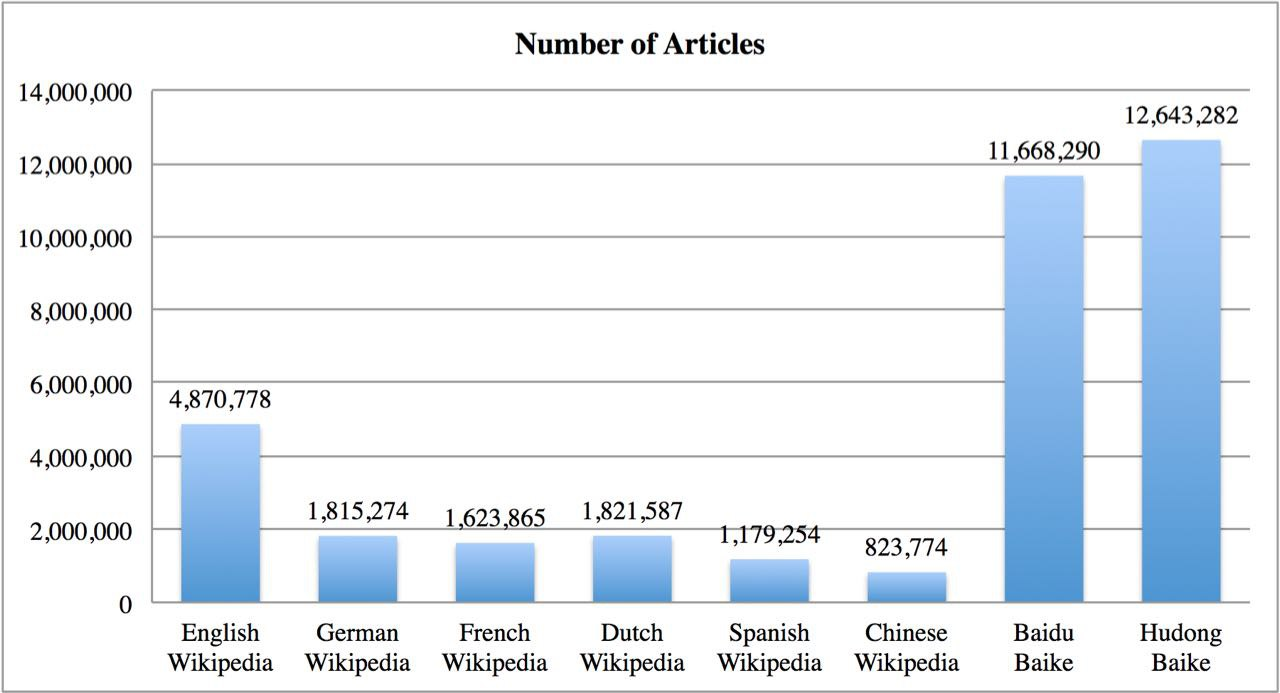
\includegraphics[width=0.75 \columnwidth]{fig/fig_stat.png}
\caption{Number of Articles on Major Wikipedias, Baidu Baike and Hudong Baike}
\label{fig_stat}
\end{figure}

To enrich the Chinese knowledge, we try to build a large-scale Chinese-English knowledge base by semantifying four heterogeneous online wikis, which are English Wikipedia, Chinese Wikipedia, Hudong Baike and Baidu Baike. This non-trivial task poses the challenges as follows:
\begin{enumerate}
  \item The cross-lingual links are highly limited inside Wikipedia. For instance, there are only 9\% Chinese-English matched articles in Wikipedia in all articles. How could we find enough Chinese-English \verb"owl:sameAs" relations?
  \item The subsumption relations of the online wikis' category systems contain lots of noise. For example, in English Wikipedia ``Wikipedia-books-on-people", which is actually \textit{subClassOf} ``Books", is taken as the sub-category of ``People" mistakenly. How could we detect those incorrect semantic relations?
\end{enumerate}

Driven by these challenges, we propose a unified framework to build a Chinese-English knowledge base from four heterogeneous online wikis. The framework contains three steps: extracting dataset from online wikis, extending an initial cross-lingual link set, and pruning taxonomy for more precise semantic relations. The generated knowledge base contains 663,740 classes, 56,449 properties and 10,856,042 instances. Specifically, we make the following contributions:
\begin{enumerate}
  \item We extend cross-lingual link set by employing a cross-lingual knowledge linking discovery approach for class and instance, and by analyzing templates in Wikipedia for property.
  \item We prune the original taxonomy, which is extracted from wiki category system, to retrieve more precise \textit{subClassOf} and \textit{instanceOf} relations.
  \item An online-system supporting keyword search and SPARQL endpoint is provided for public access to our knowledge base.
\end{enumerate}

The rest of the paper is organized as follows. Section \ref{sec:pd} presents some basic concepts and the problem formulation. In Section \ref{sec:sde} we introduce detailed extraction approaches. Section \ref{sec:cli} describes cross-lingual integration. The experimental results are reported in Section \ref{sec:result}. Related works are given in Section \ref{sec:work}. Finally we conclude our work in Section \ref{sec:con}.

\section{Preliminaries}
\label{sec:pd}
In this section, we give definitions about our knowledge base and describe our task.

%\subsection{Basic Concepts}
\para{Online Wikis.} Nowadays, Wikipedia is the largest data store of human knowledge. It was launched in 2001 and has hold over 35 million articles in 288 languages by 2015. Out of these, English articles contribute 13\% while Chinese articles account for 2\%. 

Baidu Baike and Hudong Baike are the most content-rich among the large-scale monolingual Chinese wikis currently. Hudong Baike was founded in 2005 and contains more than 12 million articles until 2015. Meanwhile, Baidu Baike maintains over 11 million articles.

Wikis usually provide two important elements with potential semantic information, category system and articles. Here, we define an encyclopedia wiki as: $W = <C,A>$, where $C$ denotes categories, $A$ denotes articles in $W$. A category system represents the relations between categories as a tree by the relation \textit{subCategoryOf}. 

\para{Wiki Pages.} Articles from the wiki sources are similar in structure. An article describes an entity with rich information. In general, six elements can be exploited in each article page:
%\begin{figure}
%    \centering
%    \begin{minipage}[t]{0.8\textwidth}
%        \centerline{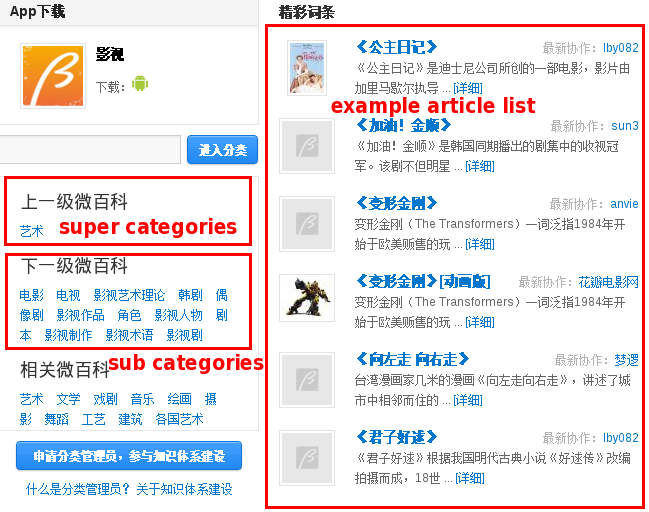
\includegraphics[width=0.8\columnwidth]{fig/hudong-taxonomy2}}
%        \caption{Taxonomy in Hudong}
%        \label{fig:hudong-taxonomy}
%    \end{minipage}%
%\end{figure}
\begin{itemize}
  \item \textbf{Title:} A Title is the label of an entity, whose uniqueness can be used to identify entities.
  \item \textbf{Abstract:} An abstract which is always the first paragraph in content, is a brief summary of the entity.
  \item \textbf{Infobox:} An infobox maintains structured data describing representative features of entity in subject-attribute-value triples.
  \item \textbf{Link:} Links are entries to other articles within the wiki. They represent the relations between the current article and others.
  \item \textbf{Category:} Categories that an article belongs to are usually listed at the bottom of article page. An article has \textit{articleOf} relation with its categories.
  \item \textbf{URL:} Each article has an HTTP url to locate itself on web.
\end{itemize}

%Fig. \ref{fig:interstellar} shows a snap of an article in Chinese Wikipedia.
%\begin{figure}[ht]
%    \centerline{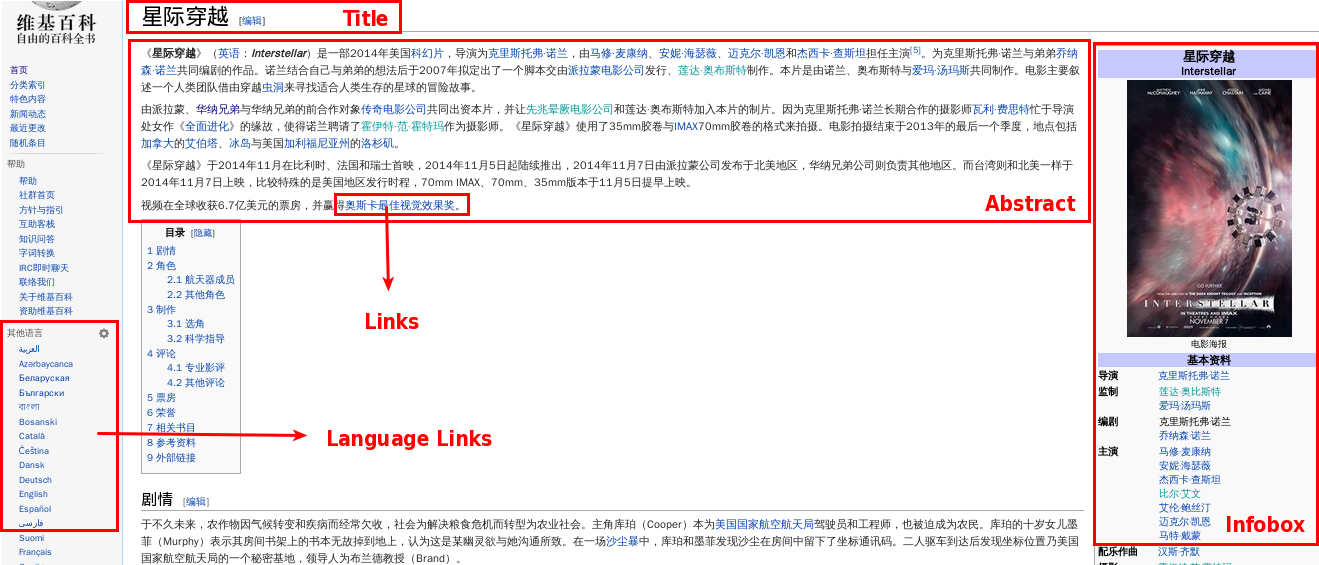
\includegraphics[width=1\columnwidth]{fig/interstellar}}
%    \caption{A snap of Interstellar(Film) article in Chinese Wikipedia}
%    \label{fig:interstellar}
%\end{figure}%
%
An article $a$ can be defined as follow:
\begin{displaymath}
    a = <Ti(a),Ab(a),Li(a),In(a),C(a),U(a)>
\end{displaymath}
where $Ti(a),Ab(a),Li(a),In(a),C(a),U(a)$ denotes title, abstract, links, infobox, category tags, url of article $a$.

Notably, infoboxes in articles are generated based on certain templates recommended by Wikipedia. An infobox template collects attributes describing similar entities. For example, content in infobox of film 冰雪奇缘(Frozen) is normalized by \emph{Template:Infobox film}, which maintains a property set of films that should be given assignment. We denote the infobox template used in article $a$ as $T(a)$. However, attribute labels in templates are usually different from those displayed on the webpage. Thus, we define an attribute as a triple $p=<tl,dl,v>$, where $tl$ is attribute label in template, $dl$ is display label in web page and $v$ is the corresponding value. The value maybe a text or a reference to another entity.

\para{Cross-lingual Links.} In Wikipedia, some article pages have cross-lingual links which help readers switch to corresponding articles in other languages. %Fig. \ref{fig:interstellar} shows language links of \emph{Interstellar} on the left column of the Wikipedia page.
As for an entity containing both Chinese article $a_{z}$ and English article $a_{e}$ in Wikipedia, we say $a_{z}$ and $a_{e}$ are \emph{cross-linked}. Infobox templates may also be cross-linked because they are articles in Wikipedia actually. For a pair $cl \in CL$, $cl = <L_{z}, L_{e}>$, where $L_{z}$ and $L_{e}$ denote the entity's cross-lingual links in Chinese and English. .

\para{Knowledge Base.} A knowledge base is a formal specification of a group of entities. Our knowledge base is described as a 4-tuple:
\begin{displaymath}
    KB = <C,P,I,H^C>
\end{displaymath}
where $C$, $P$, $I$ are the sets of classes, properties, and instances respectively. $H^C$ represents the hierarchical relationships of classes. 

Our knowledge base includes four kinds of semantic relation, which are \textit{subClassOf} of class-class, \textit{instanceOf} of instance-class, \textit{relatedClassOf} of instance and related class, \textit{relatedTopicOf} of class and related topic.

A Cross-Lingual Knowledge Base(CLKB) is a database conforming to a cross-lingual ontology. Taking advantage of cross-lingual links, several monolingual knowledge bases generated from various sources can be merge into one. Thus our Chinese-English knowledge base is defined as:
\begin{displaymath}
    CLKB = <KB_{z}, KB_{e}>
\end{displaymath}
where $KB_{z}$ and $KB_{e}$ denote the monolingual knowledge base in Chinese and English. 

\para{Cross-Lingual Knowledge Base Building.} In this paper, our task is to build a CLKB assembling knowledge from several English and Chinese wiki sources. Given an online-wiki $W_{i}$, the final output is a Chinese-English CLKB combining $KB_{z}$ and $KB_{e}$. 

Specifically, we gain dataset including class list $C_{i}$, instance list $I_{i}$, property list $P_{i}$, class hierarchical relationships $H^C_{i}$ of $W_{i}$ by extraction. We then enrich the existing cross-lingual link set $CL$ using a link-discovery method. We also refine taxonomy by checking if an \textit{articleOf} or \textit{subCategoryOf} is really an \textit{instanceOf} or \textit{subClassOf} relationship. At last the datasets in different languages are integrated by utilizing cross-lingual links in $CL$. The whole procedure is shown in Fig. \ref{fig:procedure}. 
%We extract information from four sources, Baidu Baike, Hudong Baike, Chinese Wikipedia and English Wikipedia. Because of heterogeneity, various extractors should be employed. After data parsing, we delete incorrect semantic relations by going through taxonomy pruning. At last, using the extended cross-lingual links, we combine the four dataset into our CLKB.

\begin{figure}[ht]
    \centerline{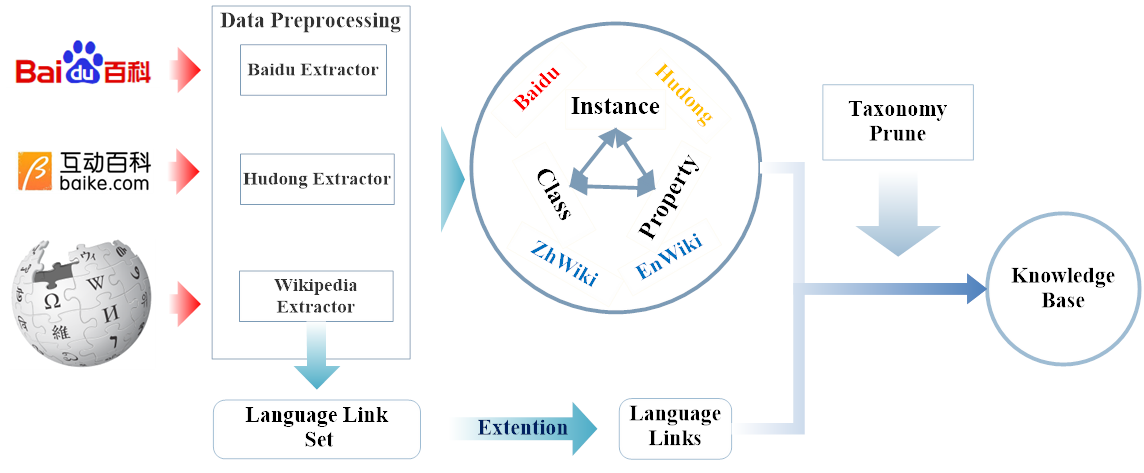
\includegraphics[width=1\columnwidth]{fig/procedure2}}
    \caption{Procedure of Building Our Cross-Lingual Knowledge Base}
    \label{fig:procedure}
\end{figure}

\section{Semantic Data Extraction}
\label{sec:sde}
Semantic data extraction aims to achieve a structured dataset from the input wikis. Specifically, we extract classes from category system, instances according to articles, and properties based on infoboxes.

\subsection{Class Extraction}
\label{sec:ce}
A class is defined as a type of similar instances. For example, the class of instance 冰雪奇缘(Frozen) is 电影(Film). In general, a class is semantic related with other classes by $subClassOf$ relation. Such relations comprise a class hierarchy $H^C$ which presents the backbone of an ontology. In a wiki, a category groups several articles and also has $subCategoryOf$ relation with others. Therefore we can extract classes based on existing category system.

However, the whole class hierarchy can not directly transform from category system due to the following problems:
\begin{itemize}
    \item There are auxiliary categories in Wikipedia, which help arrange specific articles or category pages. For example, \emph{Lists of artists} or \emph{Food templates}.
    %s\item Some sub-category links in the category system maybe inconsistent. Some categories may contain itself as sub-category, or contain sub-category that also be the super-category of it. As Fig. \ref{fig:category-mistakes} shows: In Hudong, the sub-category of 国家元首(Head of State) contains itself as a child, which causes a circle in taxonomy tree. Meanwhile, in Wikipedia, \textcolor{red}{例子}
    \item Some categories relate to only one article. According to the definition of class, such categories are less representative types, therefore it's unwise to retain them as classes.
\end{itemize}

To gain a more precise $H^C$ in a wiki, we discard categories matching the above conditions, then build the original class hierarchy $H^C$ using the remaining categories.

%However, among the relations there are still incorrect samples. \textcolor{red}{example}
%For example, \emph{Frozen} is not an entity of \emph{Disney Princess}, but relates to. Thus we will prune the taxonomy later.

\subsection{Property Extraction}
\label{sec:pe}
A property is defined as an attribute of an entity. We divide properties into two types: object property, whose value is an individual, such as 导演(directed by); datatype property, whose value is a literal text, such as 出生日期(birth date). Considering both content and infobox of an article, we extract two kinds of properties, General-properties and Infobox-properties.

\para{General-properties.} %Characteristics of an entity are regarded as general properties, including label, abstract, and url. 
General-properties describe general information of an entity. We define three datatype properties as general-properties for a given article $a$: (1) label; (2) abstract; (3) URL.

\para{Infobox-properties.} Attributes acquired from infobox are considered as infobox properties, such as 上映时间(release date), 导演(directed by) in a movie's infobox. The type of a property, datatype or object, depends on the type of its value. Ordinarily, a plain text value marks the property as datatype while an entity reference determines the property as object. For example, the attribute 上映时间(release date) can be defined as a datatype property as its value is a datetime string. On the other hand, 导演(directed by) is an object property because its value points to a person who directed the movie.

We are challenged when extracting properties from infoboxes:
\begin{itemize}
    \item In Wikipedia, because the data is from dump files published in specific XML format rather than html pages like Baidu or Hudong, the attribute label displayed in the webpage infobox is inconsistent with that in the published dump file. Fig. \ref{fig:infobox-template} gives a mapping result of display labels and dump labels in 冰雪奇缘(Frozen)'s infobox. Webpage infobox is on the left. The right is a glance from dump file in Wikipedia. The attribute label 主演 displayed on webpage is different from label \emph{starring} extracted from dump data. However, readers generally consider the display label rather than extracted label as an attribute label.
    \begin{figure}[ht]
        \centerline{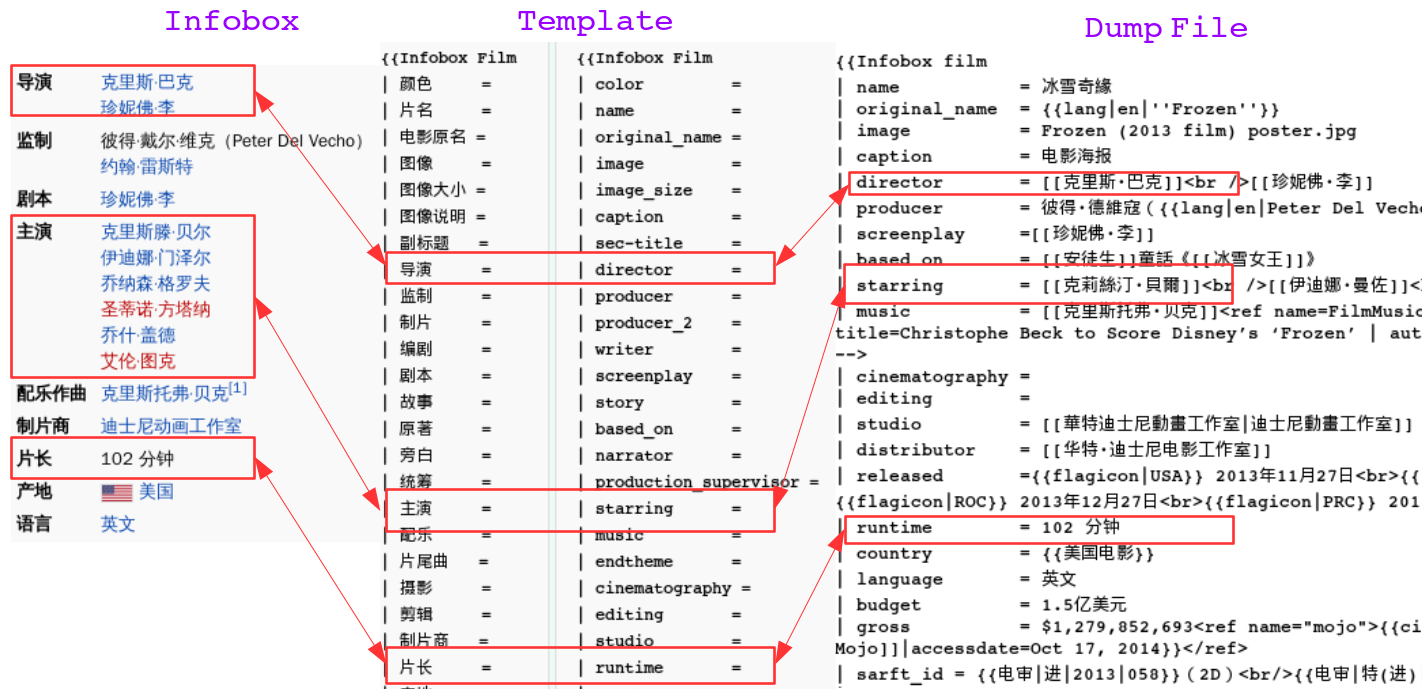
\includegraphics[width=1\columnwidth]{fig/infobox-template3}}
        \caption{Comparison of display label and dump label in \emph{Frozen} infobox}
        \label{fig:infobox-template}
    \end{figure}%
    \item There are special characters in labels. Wikipedia usually uses hyphen ``-" or dot ``•" to mark sublabels. For example, attribute 人口(population) has sub-attributes ``-Density" and ``-Urban". In addition, ``:" or ``*", may occur in Baidu or Hudong attribute labels by mistake.
\end{itemize}

To solve the problems above, we take advantage of template information. Specifically, Wikipedia institutes rules of rendering label in templates. Middle of Fig. \ref{fig:infobox-template} shows an example of \emph{Template:Infobox film}, where relations of display labels and dump labels come from. When a dump label occurs in dump file, we replace it by its mapping display label. Then we clean attribute labels to sweep incorrect characters. Furthermore, properties correspond to only one instance are discarded.

\subsection{Instance Extraction}
\label{sec:ie}
An article describes a unique entity in the world. Therefore we can extract an article as an instance. During the extraction, illustrative or structure-related articles in Wikipedia are deleted, including category list pages and template documentations.

We harvest four types of information during this stage. (1) General-properties of instance, including title as label property value, first paragraph as abstract property value and HTTP URL as URL property value; (2) Infobox-properties which are acquired via extracting from the infobox in the article; (3) $articleOf$ relation with categories listed at the bottom of article page. For example, 冰雪奇缘(Frozen) is an article of category 美国电影作品(American films); (4) Reference relation with other instances according to links in the content, such as 冰雪女王(The Snow Queen).

\section{Cross-lingual Integration}
\label{sec:cli}

To construct a CLKB with obtained structured data, firstly we argument cross-lingual links, which can help match the same entity in two languages. Secondly, we integrate four wiki datasets, that is, respectively merging classes, instances and properties from the four sources. Thirdly, we prune the taxonomy generated from class relationships to make it more accurate.

\subsection{Cross-lingual Linking}
We follow two ways to get cross-lingual links for class, instance and property. One is extracting links according to Wikipedia language links for class and instance, the other is achieving links using infobox templates for property. 

There are 227 thousand cross-lingual links between English and Chinese, which constitute the initial cross-lingual link set of classes and instances. Moreover, we utilize the language-independent method in \cite{wang2012cross} to extend the language-link set. With the linkage factor graph model, we harvest a cross-lingual links extension as many as 215 thousand with an ideal precision 85.5\% and a recall of 88.1\% between English Wikipedia and Baidu Baike.

However, due to using templates, Infobox-properties have no obvious cross-lingual links. Thus, we take the following steps to acquire property links:
\begin{enumerate}
    \item Given two cross-linked templates, $T_{e}$ and $T_{z}$, find the display labels mapping the same template label. That is, for $p_{e}$ in $T_{e}$ and $p_{z}$ in $T_{z}$, if $p_{e}.tl$ is equal to $p_{z}.tl$, $<p_{e}.dl,p_{z}.dl>$ are cross-lingual property labels;
    \item Given two cross-linked articles, $a_{e}$ and $a_{z}$, and their infobox templates, English template $T_{e}(a_{e})$ and Chinese template $T_{z}(a_{z})$, find the matched display labels mapping to the same template label;
    \item Given two cross-linked articles and their Infobox-properties $P_{e}$ and $P_{z}$, $p_{e}.dl$ and $p_{z}.dl$ are cross-lingual when: (1)for datatype properties, if $sim(p_{e}.v, p_{z}.v) > threshold$(usually useful when the value is datetime or number), where $sim(a,b)$ is a similarity calculation function. (2)for object properties, if $p_{e}.v$ and ${p_{z}.v}$ refer to the same entity. 
\end{enumerate}

In order to integrate all wikis into one, we unify classes(instances or properties) describing the same thing from four sources, and distribute a unique identifiers. For instance, we merge instances by the following steps: (1) Merge all instances extracted from wikis by title. (2) If a Chinese instance has a cross-linked English instance, that is, to an $L_{z}$, if there is $<L_{z}, L_{e}>$ in $CL$, make the two as one instance. (3) Identify all instances, including both monolingual or matched, by IDs.

The process of unifying class and property is the same as instance. Meanwhile, all the relations are kept to prevent loss of information.

\subsection{Taxonomy Prune}

%As a result of combining multi-source information without verifying, there is noise in taxonomy. %For example:
There is inevitably noise in the taxonomy since we combine multi-source information without verification. Therefore, we introduce the method from \cite{wang2014cross} to detect the correct \textit{subClassOf} and \textit{instanceOf} relations from \textit{subCategoryOf} and \textit{articleOf}. %Table. \ref{tab:} shows some examples of correct relations.
In particular, some language-dependent literal and language-independent structural features are defined to vectorize each class or instance. Employing these features, a binary-classification model is trained based on Logistic Regression. The whole process is iterative by retraining model with assured result to get higher precision. Moreover, the prediction results are validated by cross-lingual information.

The ideal result after pruning is a tree, whose edges, nodes, and leaves respectively denote semantic relations, classes and instances. However, since getting rid of incorrect entity relations without consideration of integrity, a forest result is inevitable.

To retain integrity of semantic relation, we define two types of new relations: \textit{relatedClassOf} for cut instance-class relations and \textit{relatedTopicOf} for pruned class-class relations. 

\section{Result}
\label{sec:result}
Here we show statistic results of our CLKB and introduce the system based on the knowledge base.

\subsection{Extracted Knowledge Base}
We collect the resources from four online wikis, English and Chinese Wikipedia dump files in May, 2014, Hudong html pages until May, 2014, and Baidu html pages until September, 2014. Each of the wikis has three types of information, which can be utilized for constructing our knowledge base, namely, category system, specific articles, and attributes of articles. We extract each raw data, then form the extracted information into well-structured data. Table \ref{tab:extract-result} shows the result we get after elementary extraction on 4 different wiki sources. Besides, we obtain 227 thousand class or instance links between English and Chinese in Wikipeidia, and increase the number by 215 thousand Enwiki-Baidu language links and 10 thousand property cross-lingual links.

\vspace{-0.5cm}
\begin{table}[hb]
    \small
    \centering
    \caption{Statistics of Elementary Extraction Result}
    \label{tab:extract-result}
        \begin{tabular}{|p{2.5cm}|p{2cm}|p{2cm}|p{2cm}|p{2cm}|}
            \hline
                       & Enwiki    & Zhwiki   & Hudong    & Baidu     \\ \hline
            \#Class    & 982,432   & 159,705  & 31,802    & 1300      \\ \hline
            \#Instance & 4,304,113 & 662,650  & 5,590,751 & 5,622,404 \\ \hline
            \#Property & 43,976    & 18,842   & 1187      & 139,634   \\ \hline
        \end{tabular}
\end{table}
\vspace{-0.5cm}

We create URIs \url{http://clkb/type/id} (type could be \textit{class}, \textit{instance}, \textit{property}) to identify each entry and provide corresponding information if users look up knowledge over HTTP protocol to achieve the knowledge base.

After fusing the heterogeneous sources, we harvest a cross-lingual knowledge base with 663,740 classes, 56,449 properties, and 10,856,042 instances respectively. With different methods of extraction and language link discovery, these three kinds of entries show different results in languages. We give a breakdown of both Chinese knowledge and English knowledge in Table \ref{tab:kb-result}.
\vspace{-0.5cm}
\begin{table}[ht]
\small
\centering
\caption{Statistics of Our Knowledge Base}
\label{tab:kb-result}
\begin{tabular}{|p{2cm}|p{1.5cm}|p{1.5cm}|p{1.5cm}|p{1.5cm}|p{1.5cm}|p{1.5cm}|}
\hline
\multicolumn{1}{|c|}{} & \multicolumn{2}{c|}{Classes}     & \multicolumn{2}{c|}{Instances}                   & \multicolumn{2}{c|}{Properties}    \\ \hline
English                & 639,020 & 96.26\%                & 3,879,121              & 38.79\%                & 15,380  & 27.24\%                \\ \hline
Chinese                & 88,615  & 13.35\%                & 7,409,519              & 68.25\%                & 51,618  & 91.44\%                \\ \hline
Cross-lingual          & 63,895  & 9.63\%                 & 432,598                & 3.98\%                 & 10,549  & 18.69\%                \\ \hline
English Only           & 575,125 & 86.65\%                & 3,446,523              & 31.75\%                & 4,831   & 8.56\%    \\ \hline
Chinese Only           & 24,720  & 3.72\%                 & 6,976,921              & 64,27\%                & 41,069  & 72.75\%   \\ \hline
Total                  & 663,740 & \multicolumn{1}{c|}{-} & 10,856,042             & \multicolumn{1}{c|}{-} & 56,449  & \multicolumn{1}{c|}{-} \\ \hline
\end{tabular}
\end{table}
\vspace{-0.5cm}

\subsection{Web Access to CLKB}

\begin{figure}[ht]
    \centerline{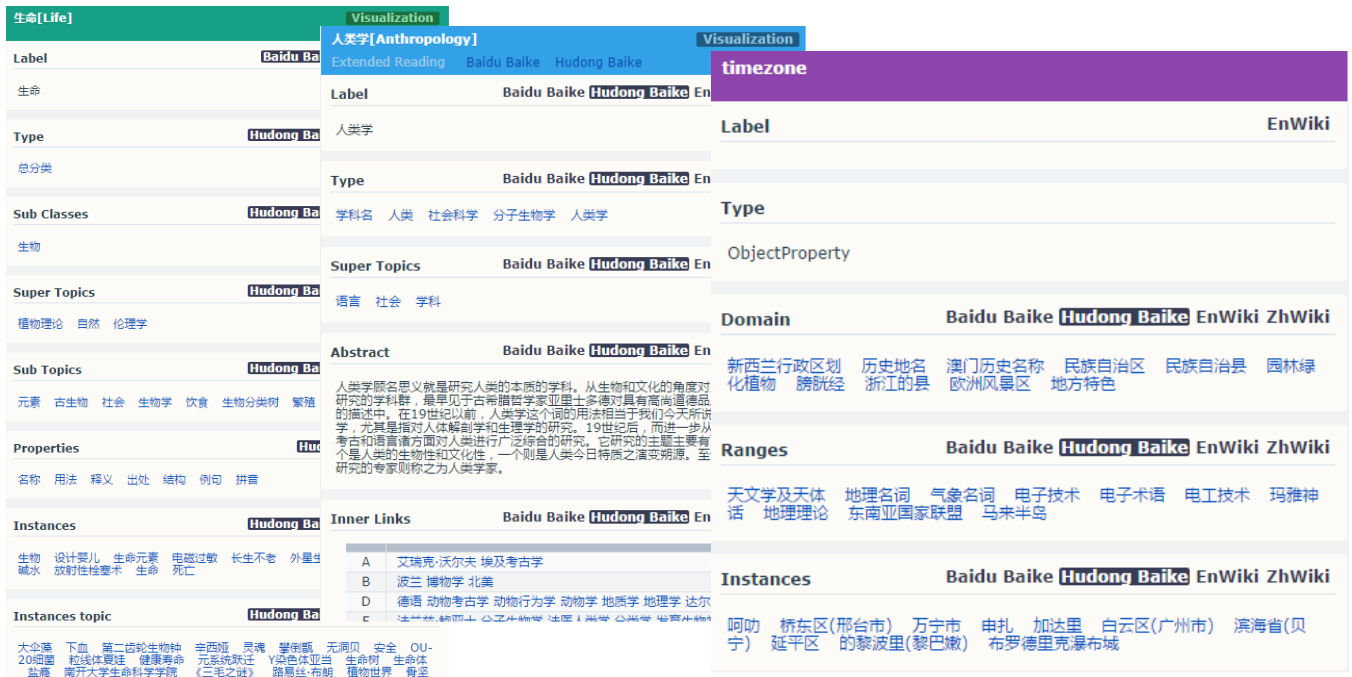
\includegraphics[width=1\columnwidth]{fig/xlore}}
    \caption{Sample Pages of Instance, Class and Property}
    \label{fig:xlore}
\end{figure}

Our knowledge base is organized in Openlink Virtuoso, which is a data management platform rendering various services, including triple store.

We provide a platform to present an intuitive visualization of our knowledge in the forms of class, instance and property. Fig. \ref{fig:xlore} shows sample pages of the integrated data. Language could be switched, which is convenient for both English speaking and Chinese speaking user. In the class webpage, we exhibit the label, super classes, subclasses, related topics, properties and instances of the specific class in bilingual way. In the instance webpage we display bilingual label, types, related classes, abstracts, infobox-properties, images and URL references. In the property webpage, we present bilingual label, type, and related instances of each property.

\begin{figure}
\centering
\subfigure[A Sample of Search Box ]{
    \label{fig:search-engine}
    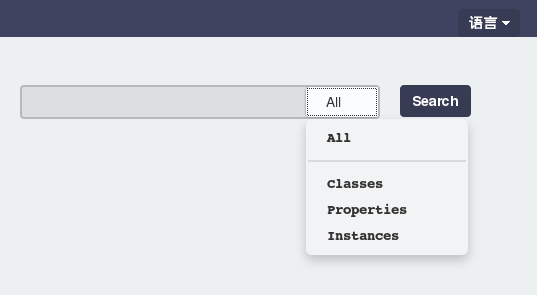
\includegraphics[width=5.5cm,height=3cm]{fig/search-engine}
    }
\hspace{0.01cm}
\subfigure[A Sample of SPARQL Query ]{
    \label{fig:sparql-endpoint}
    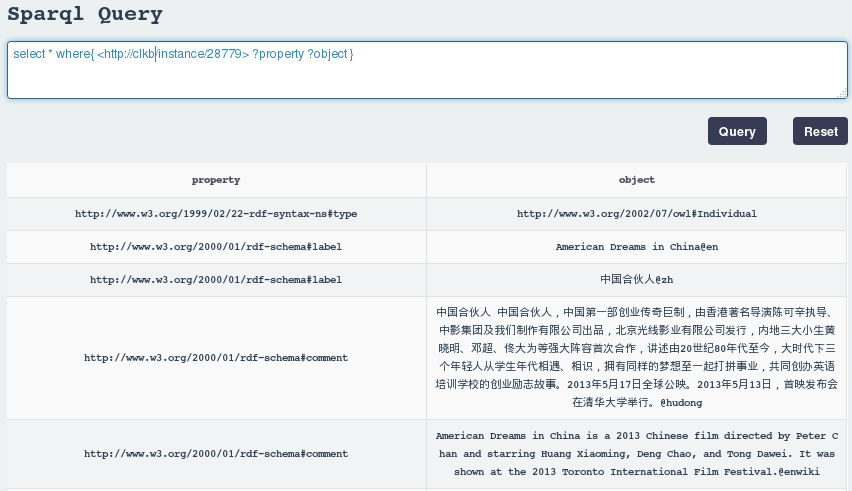
\includegraphics[width=5.5cm,height=3cm]{fig/sparql-endpoint}
    }
\caption{Two Ways Accessing to Our Knowledge Base}
\label{fig:access}
%\begin{minipage}[t]{0.5\textwidth}
%    \centerline{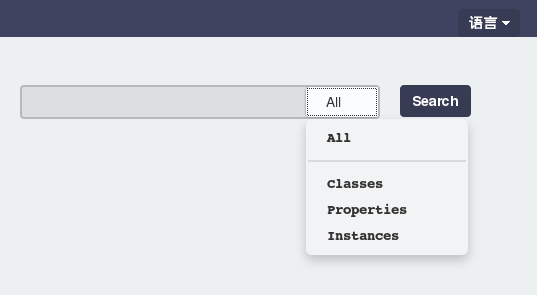
\includegraphics[width=5.5cm,height=3cm]{fig/search-engine}}
%    \caption{A picture of Search Box}
%    \label{fig:search-engine}
%\end{minipage}%
%\begin{minipage}[t]{0.5\textwidth}
%    \centerline{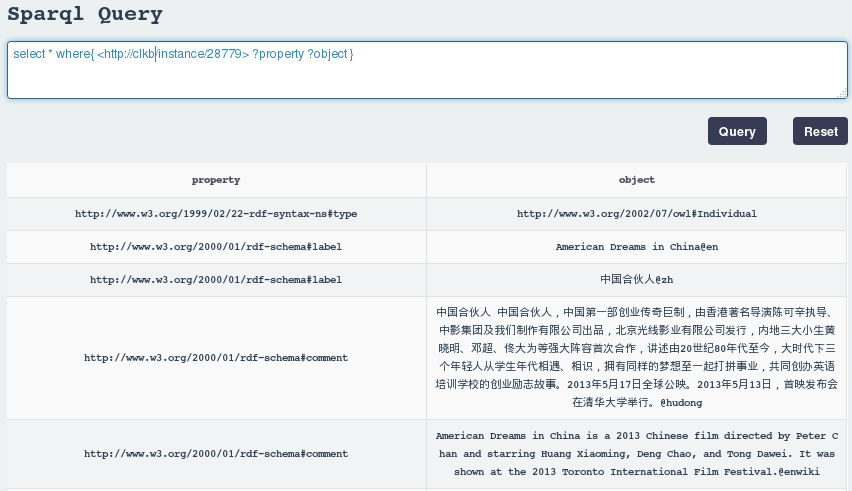
\includegraphics[width=5.5cm,height=3cm]{fig/sparql-endpoint}}
%    \caption{A SPARQL Sample Query}
%    \label{fig:sparql-endpoint}
%\end{minipage}%
\end{figure}

Beside these user-friendly pages, we provide two ways to access our knowledge base shown in Fig. \ref{fig:access}: via the search engine or via SPARQL endpoint. For general users, they can make a query by inputing related text into searchbox to get probable related entities. To present practicable result, An index is generated over all entities. We as well provide SPARQL interface for professional users to query our knowledge graph. Users can choose the language tags of their desired results by \textbf{``filter(langMatches(?label),``en"))"} or \textbf{``filter(langMatches (?label),``zh"))"}.%For example, to get the English label of an instance, the query is: select * where {$<$\url{http://clkb/instance/100}$>$ $<$\url{http://www.w3.org/2000/01/rdf-schema#label}$>$ ?label. filter(langMatches(?label),"en"))}.


\section{Related Work}
\label{sec:work}
In this section, we introduce some related knowledge bases. %and cross-lingual knowledge linking methods.

\para{Chinese Knowledge Bases.} Currently, several large-scale Chinese knowledge bases have been generated. Zhishi.me\cite{niu2011zhishi,wang2014publishing} is the first published Chinese large-scale Linking Open Data. It acquires structural information from three original sources, Chinese Wikipedia, Baidu Baike and Hudong Baike and gains more than 5 million distinct entities. Zhishi.me helps generate knowledge base focused on relations in Junfeng Pan's work\cite{pan2012building}.

Similar to Zhishi.me, CKB\cite{wang2012building} is created from Hudong Baike. It first learns an ontology based on category system and properties, and then collects 19,542 classes, 2,381 properties, 802,593 instances. Besides using existing online-wikis, CASIA-KB employs other types of sources(e.g. microblog posts, news pages, images) to enrich the structured knowledge.

\para{Cross-lingual Knowledge Bases.} DBpedia \cite{auer2007dbpedia,mendes2012dbpedia} is one of the most used cross-lingual knowledge base in the world. It extracts various kinds of structured information from Wikipedia and employs the multi-lingual characteristic of Wikipedia to generate 97 language versions of content. This knowledge base is widely applied in many domains, including media recommendation \cite{fernandez2011generic,kaminskas2012knowledge}, entity linking\cite{mendes2011evaluating} and information extraction \cite{dutta2013integrating}. 

Universal WordNet(UWN)\cite{de2012uwn} is a large multi-lingual lexical knowledge base which is built from WordNet and enrich entities from Wikipedia. It is constructed using sophisticated knowledge extraction, link prediction, information integration, and taxonomy induction methods. The API accesses to more than 16 million words and names in over 200 languages. UWN provides semantic relationship of list of word meanings for Aya's work on classual search \cite{al2015conceptual}.

%\subsection{Cross-lingual Knowledge Linking}
%Discovering more cross-lingual links is benefit to development of a multi-lingual knowledge base. General method is divided into two steps. First find missing link candidates using link structure of articles and then decide whether candidates are cross links or not by classification. \cite{sorg2008enriching} employs such approach to resolve the problem of automatically inducing new cross-language links. Wang\cite{wang2012cross} utilize a linkage factor graph model

\section{Conclusion}
\label{sec:con}
This paper presents a procedure of building a Chinese-English CLKB from four wiki sources. At first, we extract structured information and unify data format. Then a cross-lingual link set is generated and expanded to help combine the bilingual sources. To refine our dataset, we also conduct pruning work on taxonomy. Finally, we acquire a CLKB containing 663,740 classes, 56,449 properties, and 10,856,042 instances. Currently, an online-system supporting keyword search and SPARQL query is provided to access the knowledge base.

%\section*{Acknowledgement}
%Thanks anonymous reviewers for their valuable suggestions that help us improve the quality of the paper. Thanks Prof. Chua Tat-Seng from National University of Singapore for discussion. The work is supported by 973 Program (No. 2014CB340504 ), NSFC-ANR (No. 61261130588), Tsinghua University Initiative Scientific Research Program (No. 20131089256) and THU-NUS NExT Co-Lab.

\bibliographystyle{splncs03}
\bibliography{paper}

%\end{CJK*}
\end{document}

